\chapter{Oracle Aplication Express}

\section{Tahapan Pembuatan Aplikasi Oracle Apex}
Langkah pertama yang harus dilakukan adalah membuka website https://apex.oracle.com\cite{OracleApex}. Disini kita akan mendapatkan akses untuk memasuki Oracle Apllication Express, pastikan email yang dimasukkan valid untuk membuat Workspace, berikut adalah langkah langkah pembuatan Aplikasi pada Oracle APEX :

\begin{enumerate}
\item[1]Pergi ke Website Oracle APEX, https://apex.oracle.com, lalu klik Sign In.

\begin{figure}[!htbp]
    \begin{center}
    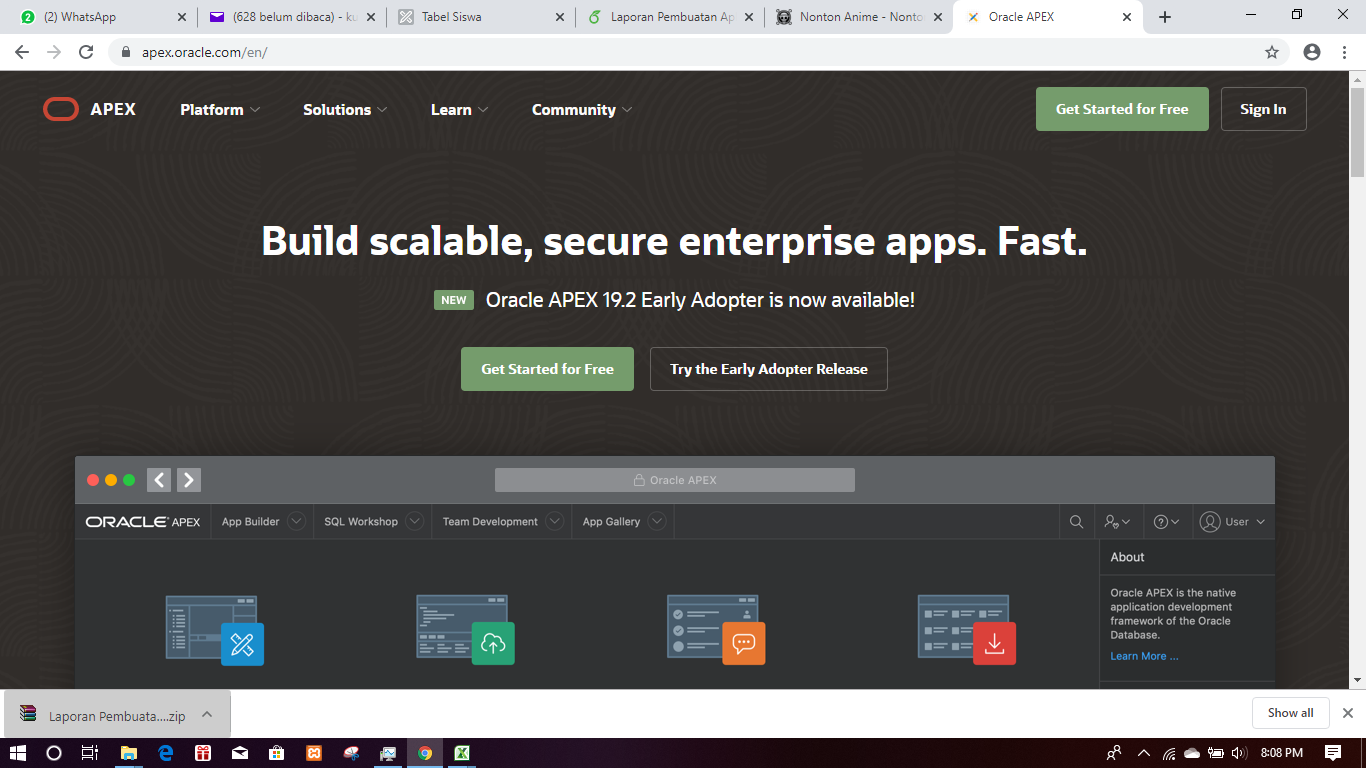
\includegraphics[scale=0.2]{figures/1.png}
    \caption{\textit{Sign In.}}
    \end{center}   
    \end{figure}
    
\begin{figure}[!htbp]
\item[2]Lalu Pergi ke klik App Builder.

    \begin{center}
    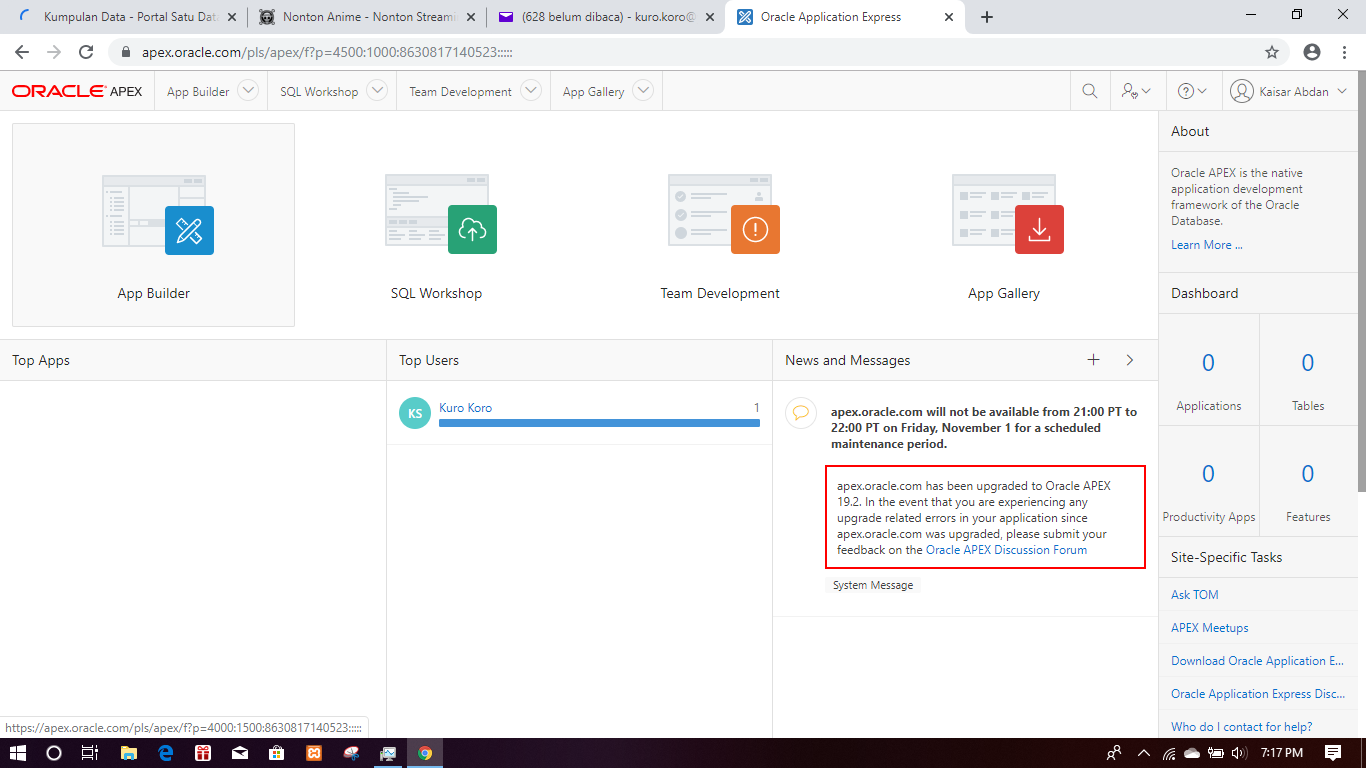
\includegraphics[scale=0.2]{figures/2.png}
    \caption{\textit{Sign In Workspace.}}
    \end{center}


\item[3] Lalu setelah itu akan muncul create, kemudian klik

    \begin{center}
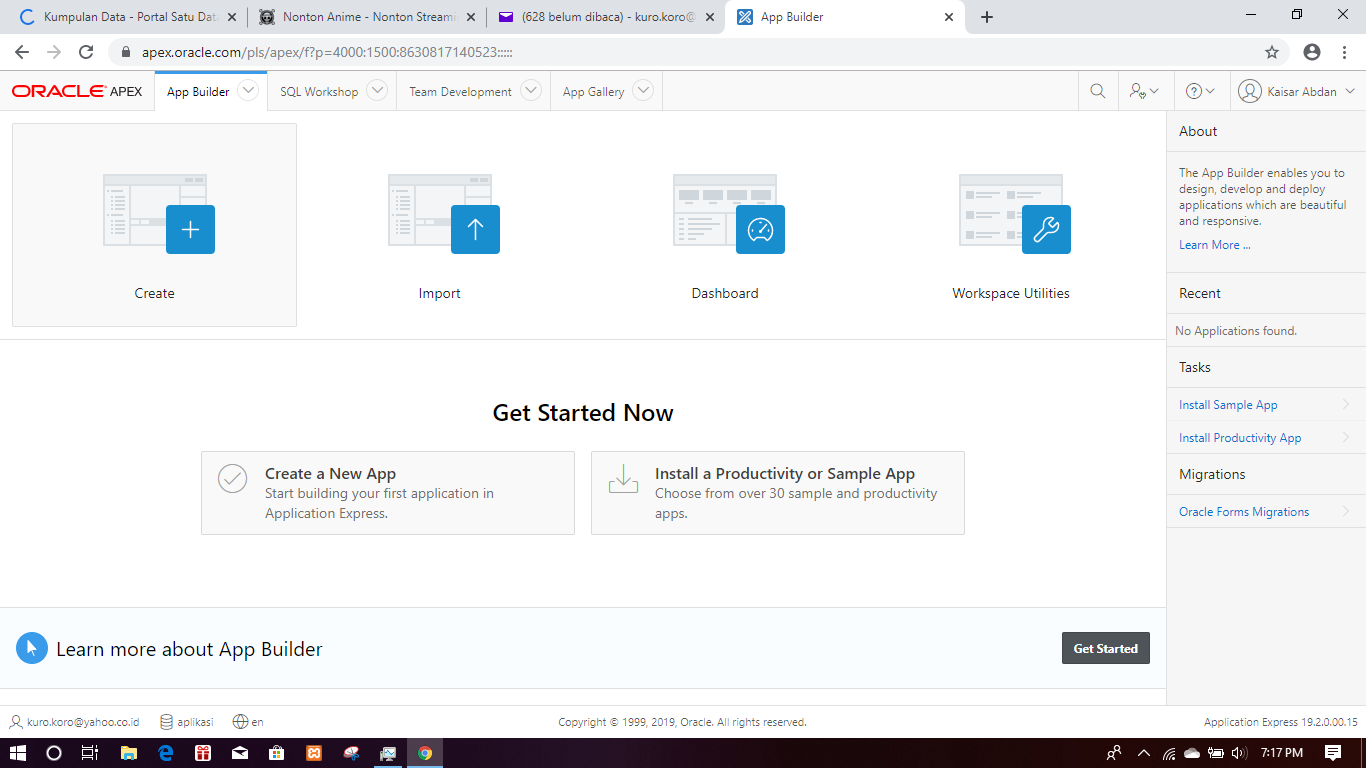
\includegraphics[scale=0.2]{figures/3.png}
    \caption{\textit{App Builder}}
        \end{center}
\label{gambar}
\end{figure}

\begin{figure}
\item[4] Setelah di klik create, kemudian klik From a File.

    \begin{center}
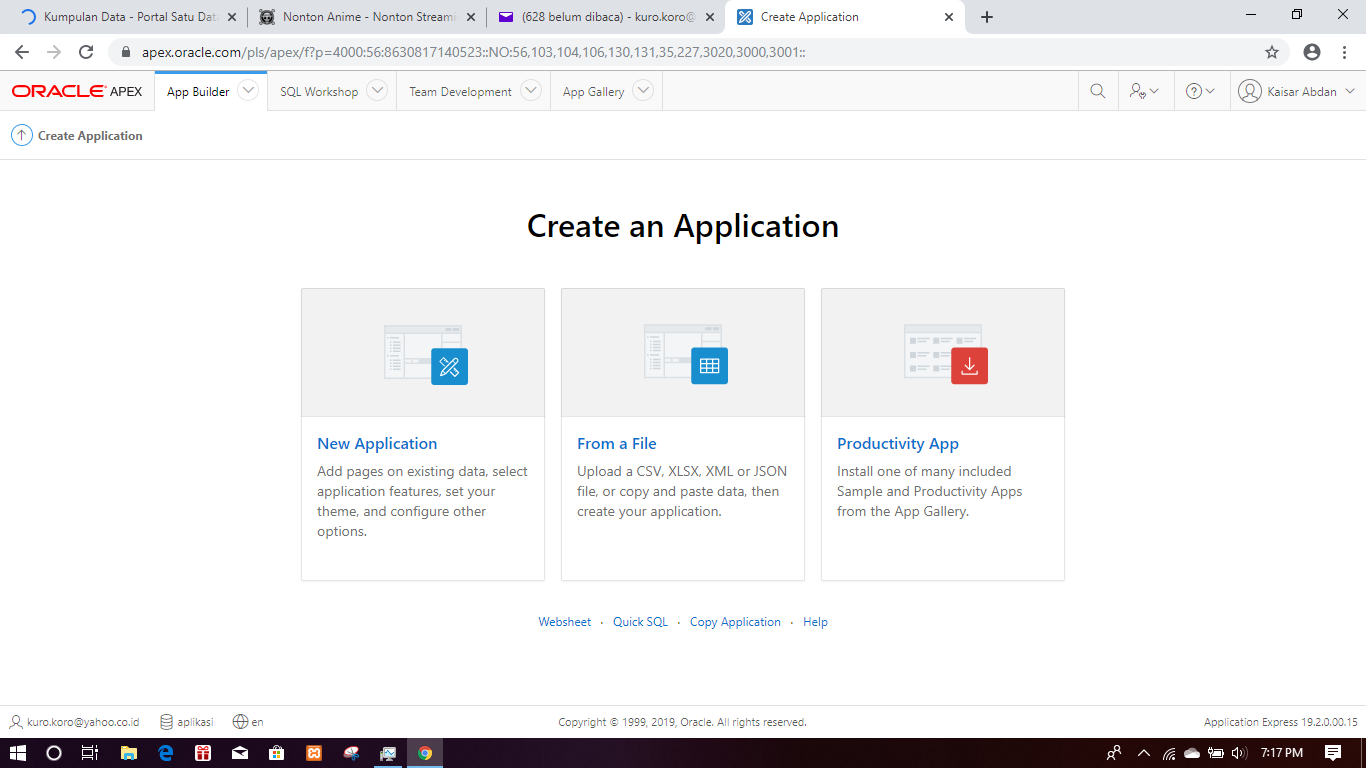
\includegraphics[scale=0.2]{figures/4.png}
    \caption{\textit{Create .}}
        \end{center}
\label{gambar}
\end{figure}

\begin{figure}
\item[5] Setelah di klik From a File, Kemudian Lakukan Drag and Drop.

    \begin{center}
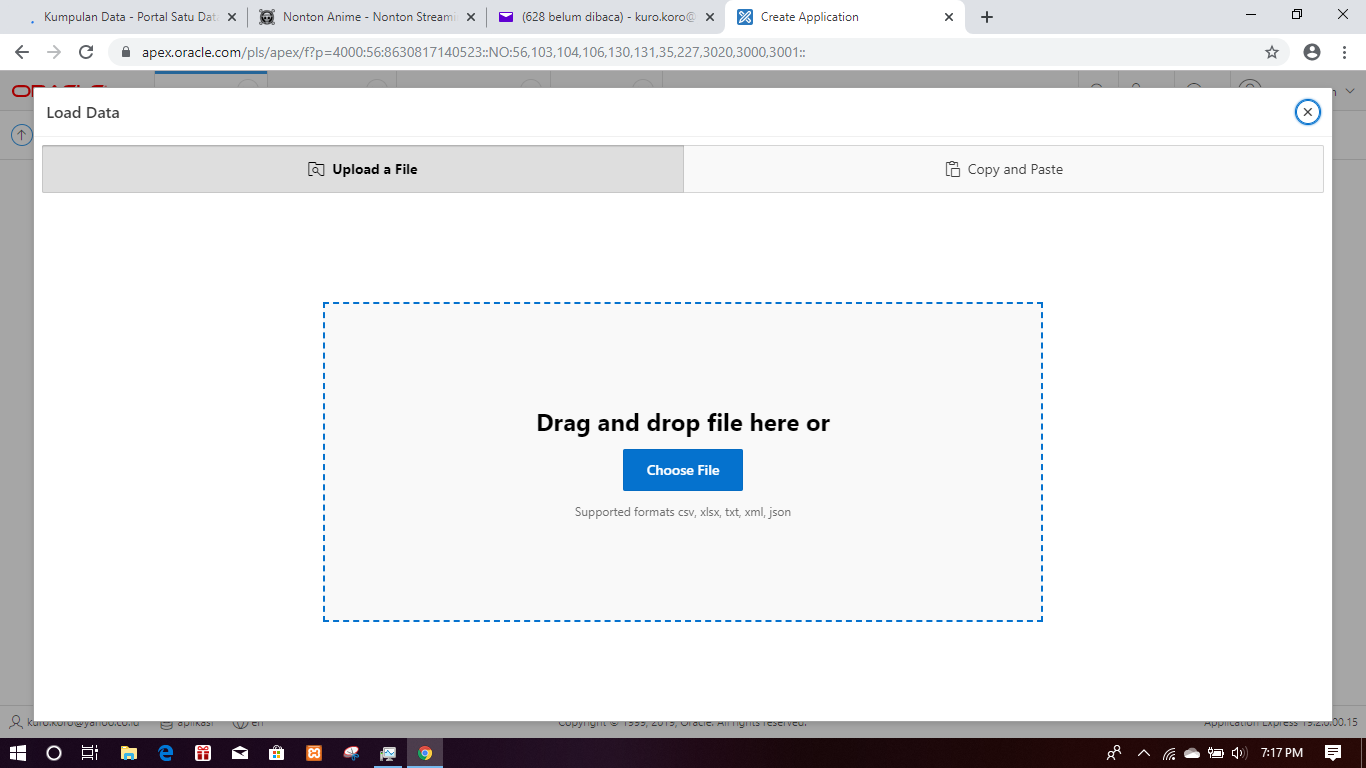
\includegraphics[scale=0.2]{figures/5.png}
    \caption{\textit{{Proses Input Data Excel}l}}
        \end{center}
\label{gambar}
\end{figure}

\begin{figure}
\item[6] Masukan data excel yang akan digunakan untuk membuat aplikasi.

    \begin{center}
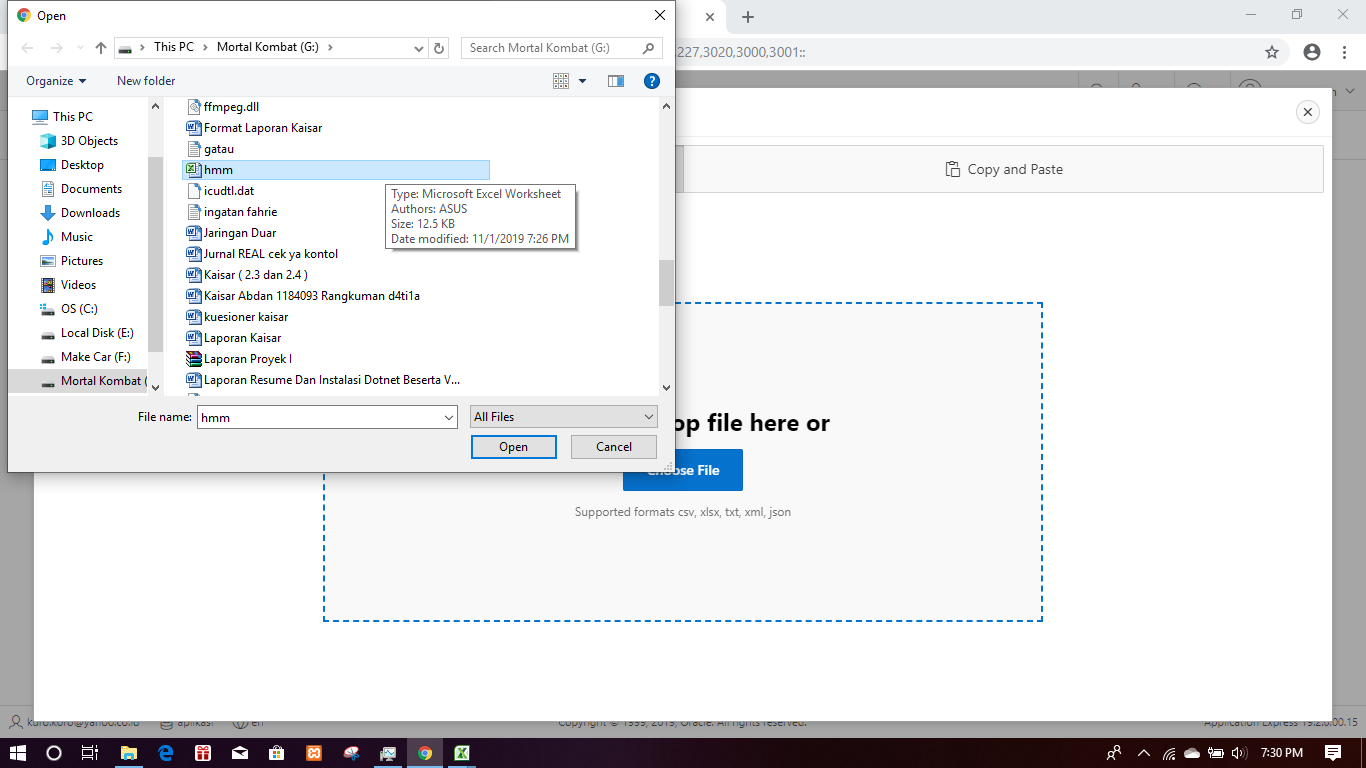
\includegraphics[scale=0.2]{figures/6.png}
    \caption{\textit{Input Data Excel.}}
        \end{center}
\label{gambar}
\end{figure}

\begin{figure}
\item[7] Lalu Muncul Tampilan seperti ini. Di Table Nama saya beri TABEL SISWA.

    \begin{center}
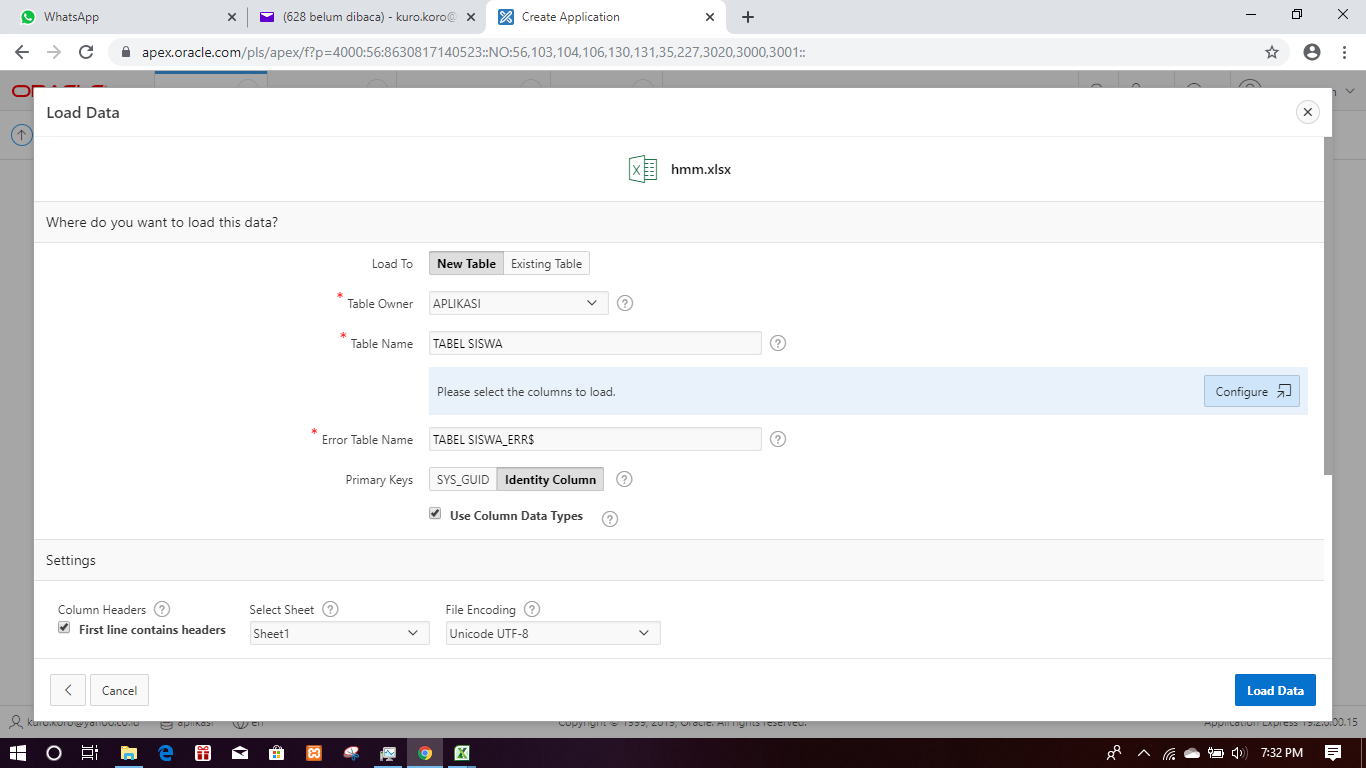
\includegraphics[scale=0.2]{figures/7.png}
    \caption{\textit{Pengisian Nama Table}}
        \end{center}
\label{gambar}
\end{figure}

\begin{figure}
\item[8] Proses Pembuatan Aplikasi Berhasil.

    \begin{center}
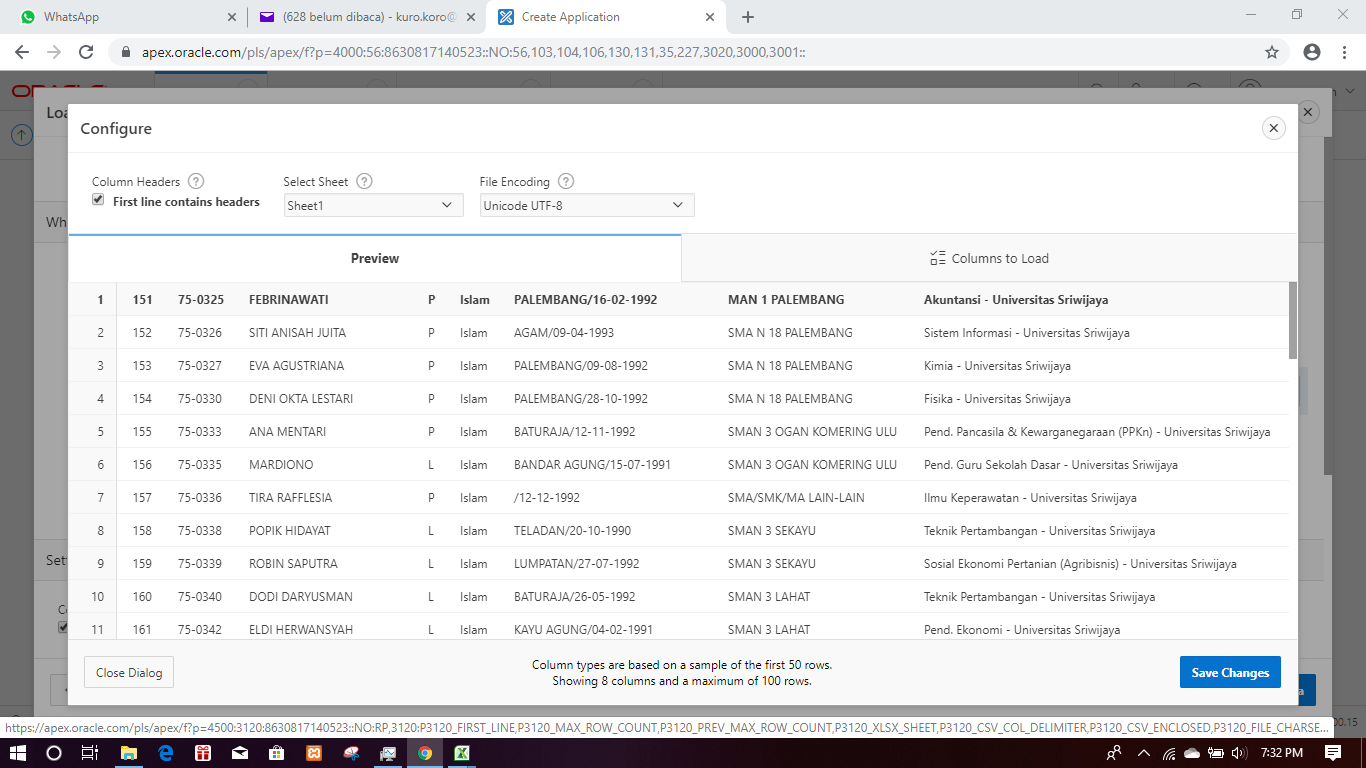
\includegraphics[scale=0.2]{figures/8.png}
    \caption{\textit{Aplikasi Berhasil}}
        \end{center}
\label{gambar}
\end{figure}

\begin{figure}
\item[9] Lalu muncul tampilan seperti ini.

    \begin{center}
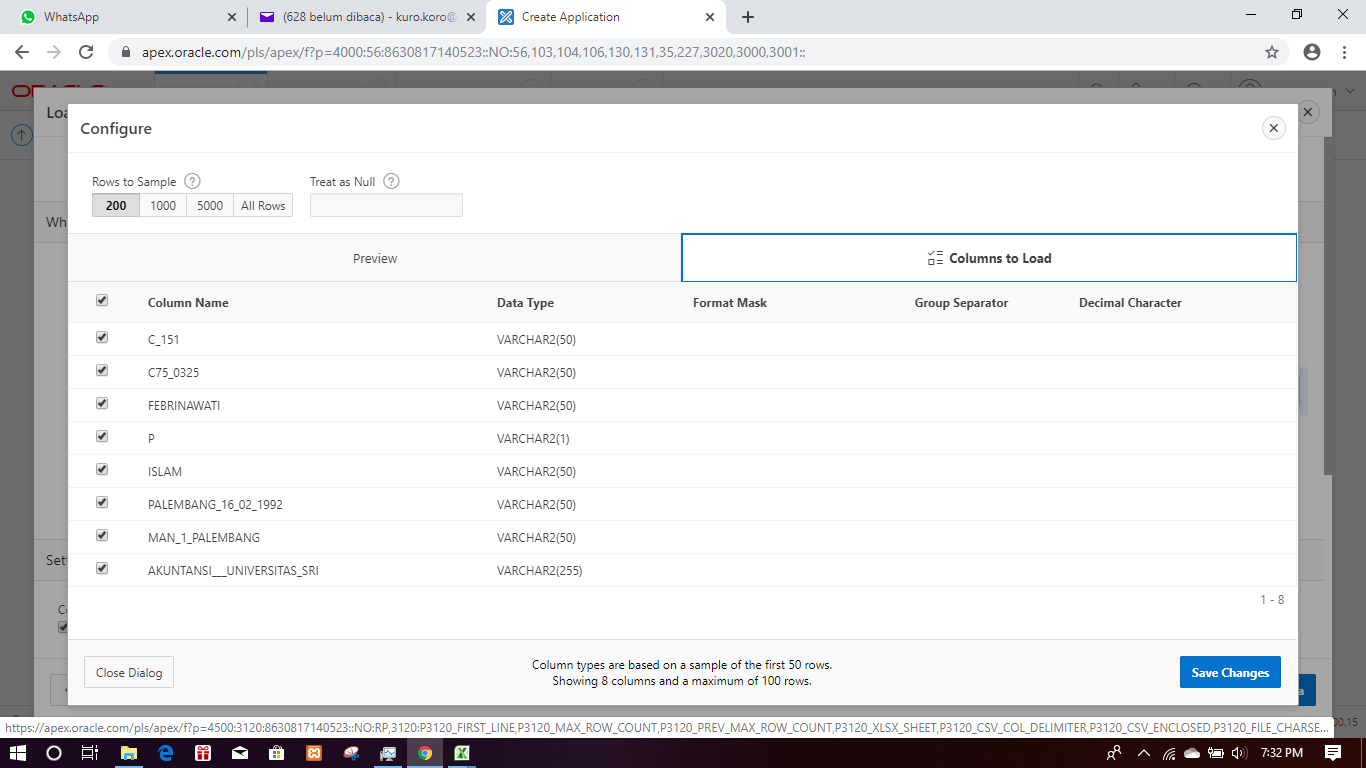
\includegraphics[scale=0.2]{figures/9.png}
    \caption{\textit{Tampilan Create Application}}
        \end{center}
\label{gambar}
\end{figure}

\begin{figure}
\item[10] Klik Run Application .

    \begin{center}
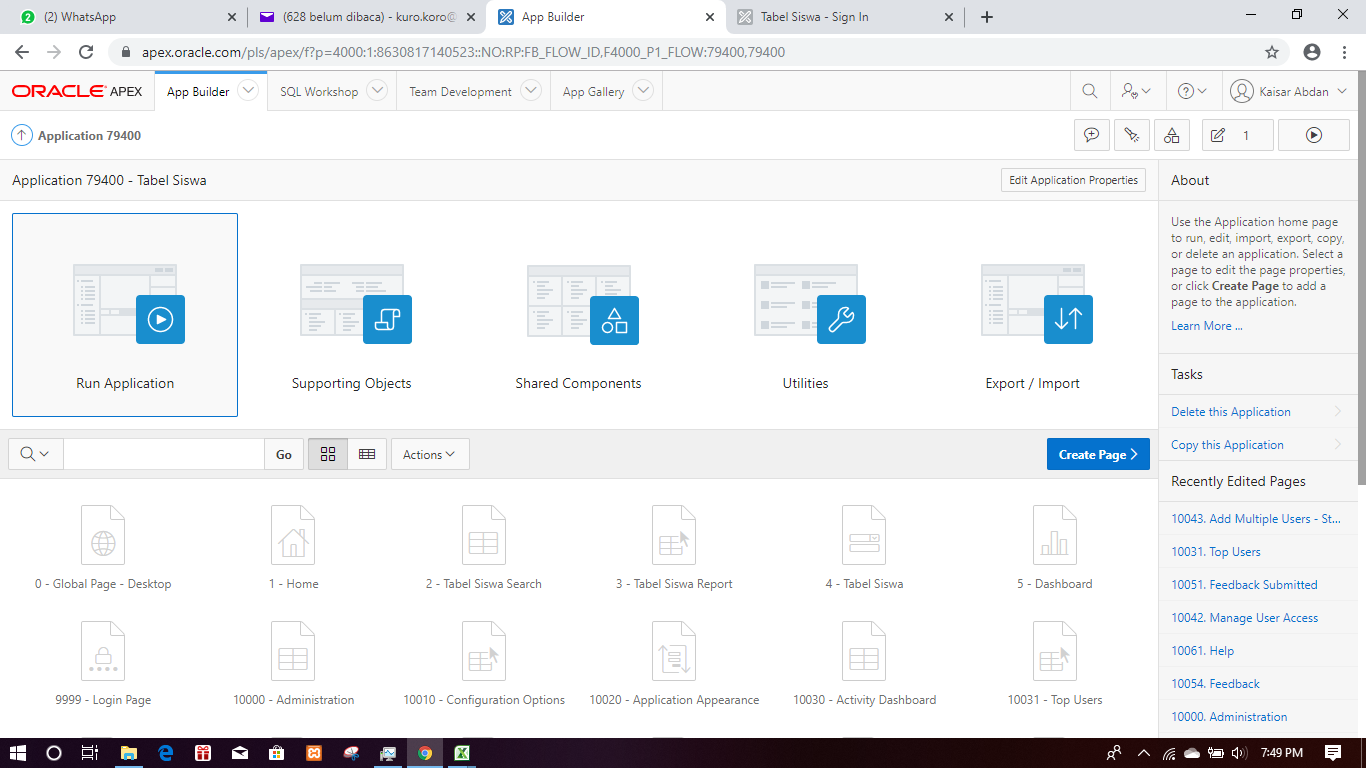
\includegraphics[scale=0.2]{figures/10.png}
    \caption{\textit{Create Application}}
        \end{center}
\label{gambar}
\end{figure}

\begin{figure}
\item[11] Lalu Create Application.
    \begin{center}
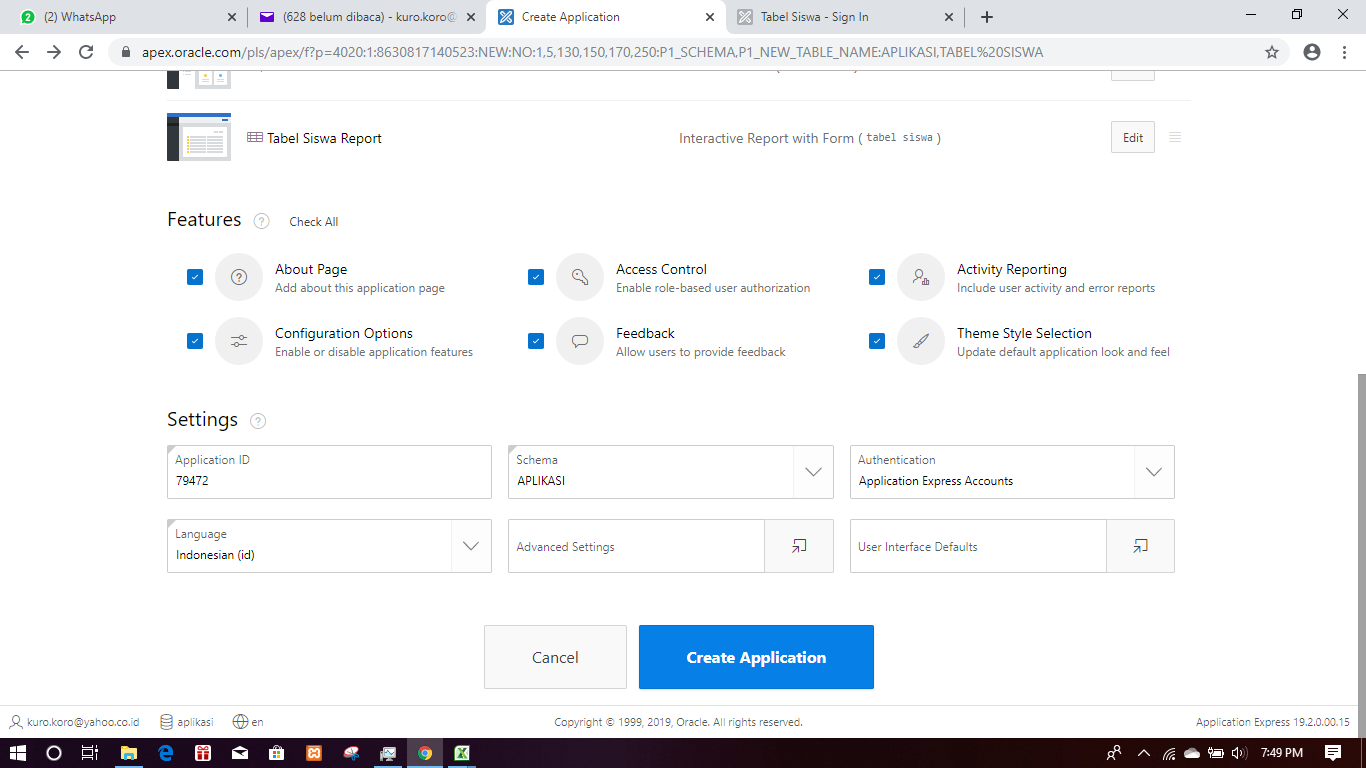
\includegraphics[scale=0.2]{figures/11.png}
    \caption{\textit{Run}}
        \end{center}
\label{gambar}
\end{figure}

\begin{figure}
\item[12] Lalu Masukan email sama password yang telah dibuat.

    \begin{center}
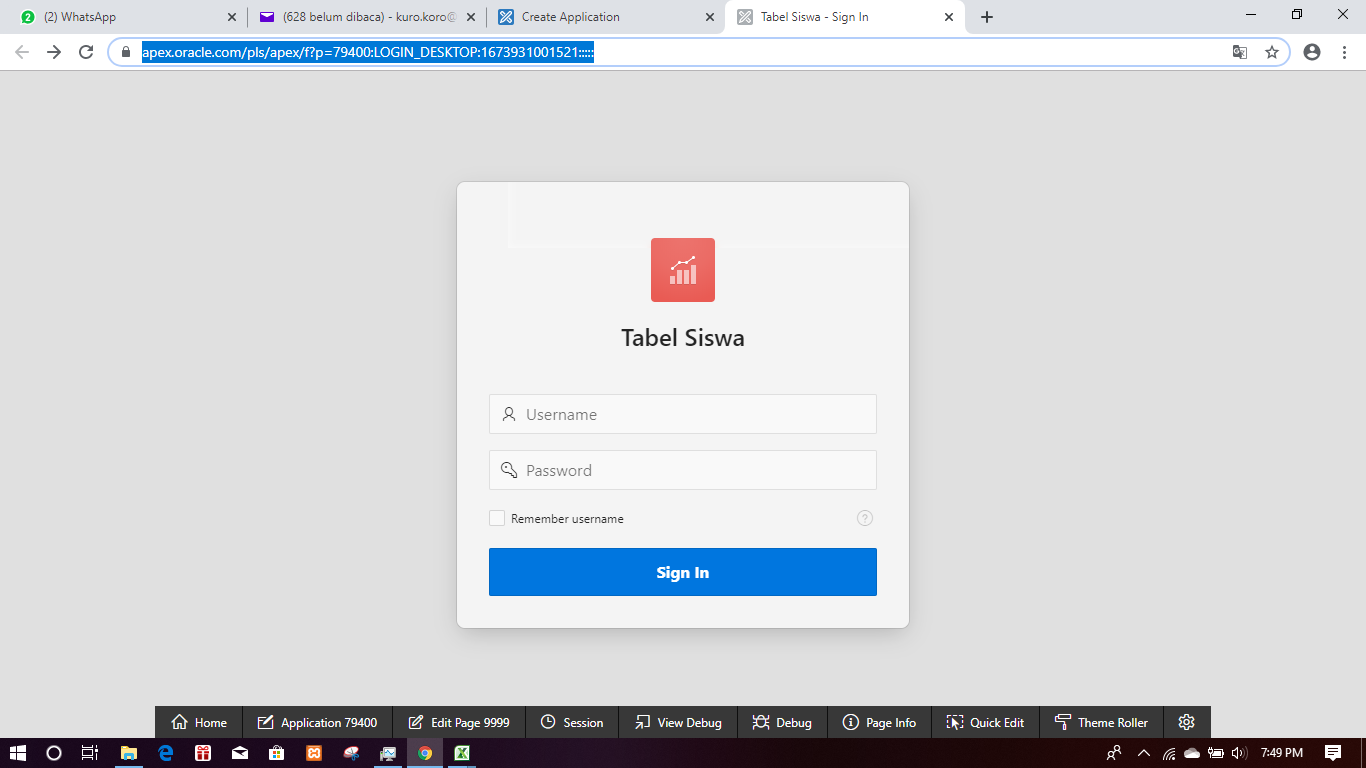
\includegraphics[scale=0.2]{figures/12.png}
    \caption{\textit{Masukan Email}}
        \end{center}
\label{gambar}
\end{figure}

\begin{figure}
\item[13] Lalu muncul tampilan seperti ini.

    \begin{center}
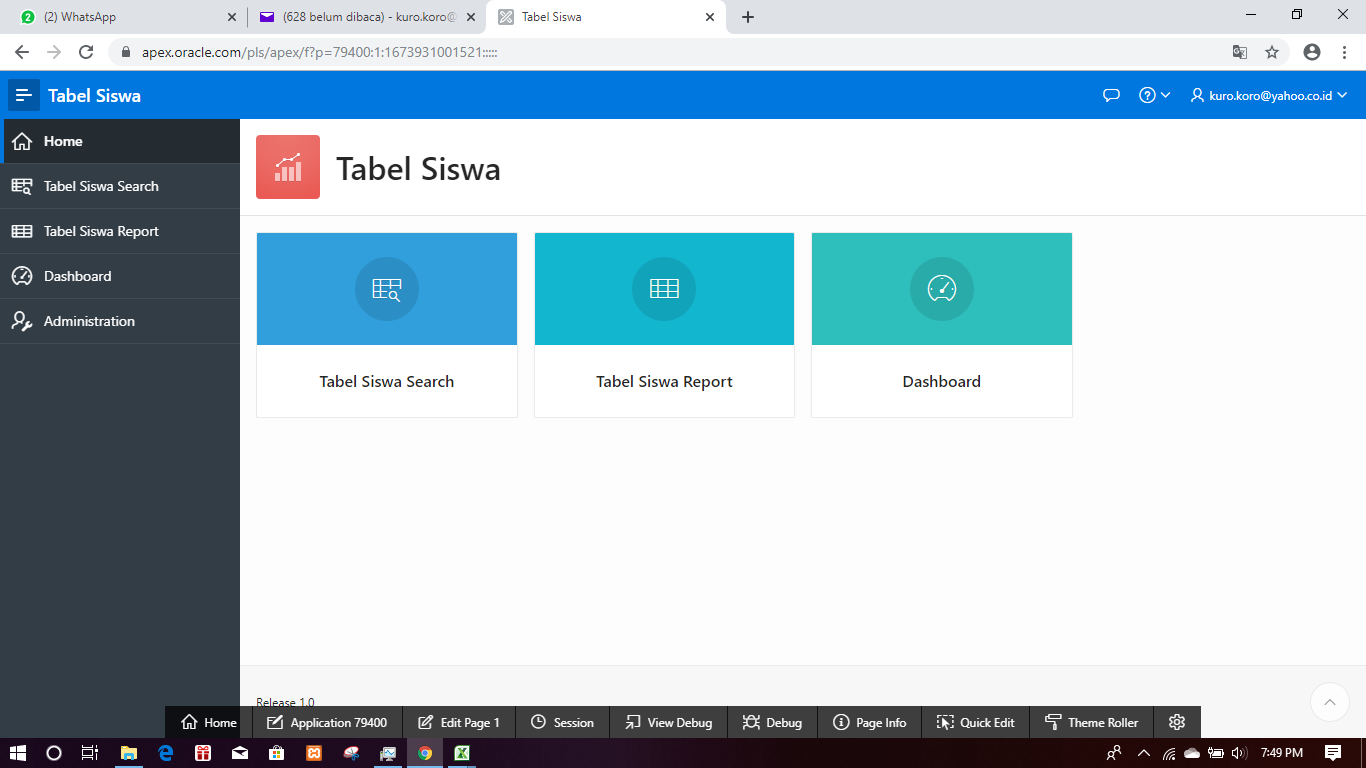
\includegraphics[scale=0.2]{figures/13.png}
    \caption{\textit{Tampilan Berhasil.}}
        \end{center}
\label{gambar}
\end{figure}


\begin{figure}

\item[14] Link Akses  https://apex.oracle.com/pls/apex/f?p=79400:1:1673931001521:::::
\item[15] username   : kuro.koro@yahoo.co.id
\item[16] kata sandi : 223790549Ka
\end{figure}

\end{enumerate}
